\documentclass[border=0.5mm]{standalone}

\usepackage{import}
\subimport{../../../}{preamble.tex}

\usepackage{tikz}
\usetikzlibrary{calc}

\usepackage{pgfplots}
\usepgfplotslibrary{fillbetween}

\begin{document}

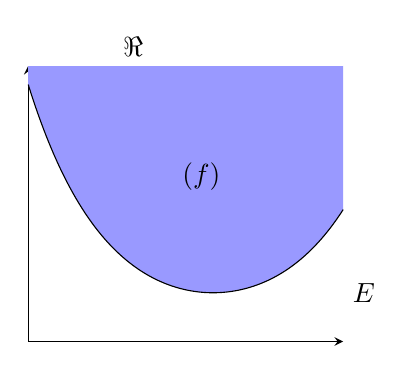
\begin{tikzpicture}

  \begin{axis}[
    ticks=none,
    axis lines=left,
    y=3.5cm,            % y unit vector
    x=1cm,            % x unit vector
    xmin=-2,
    xmax=2,
    ymin=0,
    ymax=1,
    clip=false,
    xlabel=$E$,
    ylabel=$\Re$,
    x label style={at={(axis description cs:1.0,0.175)},anchor=west},
    y label style={at={(axis description cs:0.27,1.0)},rotate=-90,anchor=south west},
    ]
    
    \addplot[name path=F, mark=none, black, samples=100, domain=-2:2] {(exp(-x)+exp(x)/2)/8};
    \addplot[name path=S, mark=none, draw=white, samples=10, domain=-2:2] {1};

    \addplot[blue!40] fill between[of=F and S];

    \node at (axis cs:0.2,0.6) {$\epi(f)$};
    
  \end{axis}

  
\end{tikzpicture}

\end{document}

%%% Local Variables:
%%% mode: latex
%%% TeX-master: t
%%% End:
